\documentclass[11pt]{article}

\usepackage[margin=0.75in]{geometry}
\usepackage{amsmath}
\usepackage{array}
\usepackage{booktabs}
\usepackage{float}
\usepackage{graphicx}
\usepackage{hyperref}
\usepackage{xcolor}
\usepackage{url}

\hypersetup{
  colorlinks=true,
  linkcolor=blue!55!black,
  urlcolor=blue!55!black,
  citecolor=blue!55!black
}

\title{Yichao Per-Z Brightfield-to-Fluorescence Performance Report}
\author{OrganoidAgent}
\date{May 20, 2026}

\begin{document}
\maketitle

\section*{Executive Summary}

This report documents the completed Yichao per-z brightfield-to-fluorescence (B2F) experiment. The task is to predict a cleaned fluorescence-derived target from the corresponding brightfield organoid crop. The model was trained on Data-Yichao-1 through Data-Yichao-10 and evaluated on Data-Yichao-11 as a strict external holdout. Data-Yichao-11 was not used for training, validation, or checkpoint selection.

The most intuitive external performance number is fluorescent-region F1. On Data-Yichao-11, the per-z model achieved support-best F1 \(=0.454\) and fixed-threshold F1 \(=0.418\). The positive support prevalence in Data-Yichao-11 is approximately \(0.071\), so the F1 is not a random-guess result. The model also predicted total fluorescence at \(1.135\times\) the true total, meaning the external total signal scale was about \(13.5\%\) high. Pixel-perfect reconstruction is not solved, but the model has learned real brightfield-associated signal.

\section*{Task Definition}

The target is derived from fluorescence, not brightfield. In the Yichao image convention used here, channel \(c1\) is brightfield and channel \(c0\) is fluorescence. For each segmented organoid instance:
\[
B_i = \text{brightfield crop}, \quad
F_i = \text{raw fluorescence crop}, \quad
Y_i = \text{cleaned continuous fluorescence target}.
\]
The model predicts a one-channel continuous target:
\[
\hat{Y}_i = G_\theta(B_i, M_i, D_i),
\]
where \(M_i\) is the organoid segmentation mask and \(D_i\) is an organoid distance-map auxiliary channel. The binary fluorescence support mask \(S_i\) is derived from \(Y_i\) and is used for support losses and metrics. It is not a brightfield mask.

\begin{figure}[H]
  \centering
  \fbox{\begin{minipage}{0.92\textwidth}
  \[
  \text{Brightfield }(c1) + \text{organoid mask} + \text{distance map}
  \;\xrightarrow{\text{hybrid U-Net}}\;
  \text{one-channel cleaned fluorescence target from }c0
  \]
  \[
  \text{continuous target learns intensity; support losses learn sparse positive fluorescent regions}
  \]
  \end{minipage}}
  \caption{B2F task flow. The model input is brightfield morphology plus segmentation-derived auxiliary channels. The output is a fluorescence-derived continuous target.}
\end{figure}

\section*{Data}

The main run treats every original z-plane as a separate example. No z projection is used. This preserves depth information for later time/depth modeling. A max-brightfield/max-fluorescence projection run is included as a secondary comparison because it gives a useful external performance reference.

\begin{table}[H]
  \centering
  \caption{Dataset and split counts. Data-Yichao-11 is external only.}
  \resizebox{\textwidth}{!}{\begin{tabular}{@{}llr@{}}
\toprule
Dataset stage & Definition & Count \\
\midrule
Per-z source images & Brightfield/fluorescence image records, Data 1--11 database & 79,405 \\
Per-z instance records & Segmented organoid instance records, Data 1--11 database & 354,797 \\
Per-z edge-padded instances & Instances touching crop/image boundary & 132,997 \\
Per-z usable targets & Filtered Data 1--10 rows used for target construction & 214,311 \\
Training rows & Data 1--10 train split & 139,935 \\
Validation rows & Data 1--10 validation split & 62,814 \\
Internal test rows & Data 1--10 internal test split & 11,562 \\
External rows & Data-Yichao-11 only, never used in training & 7,489 \\
\midrule
Max-projection usable targets & Data 1--10 projected rows & 9,775 \\
Max-projection external rows & Data-Yichao-11 projected rows & 420 \\
\bottomrule
\end{tabular}
}
\end{table}

\begin{figure}[H]
  \centering
  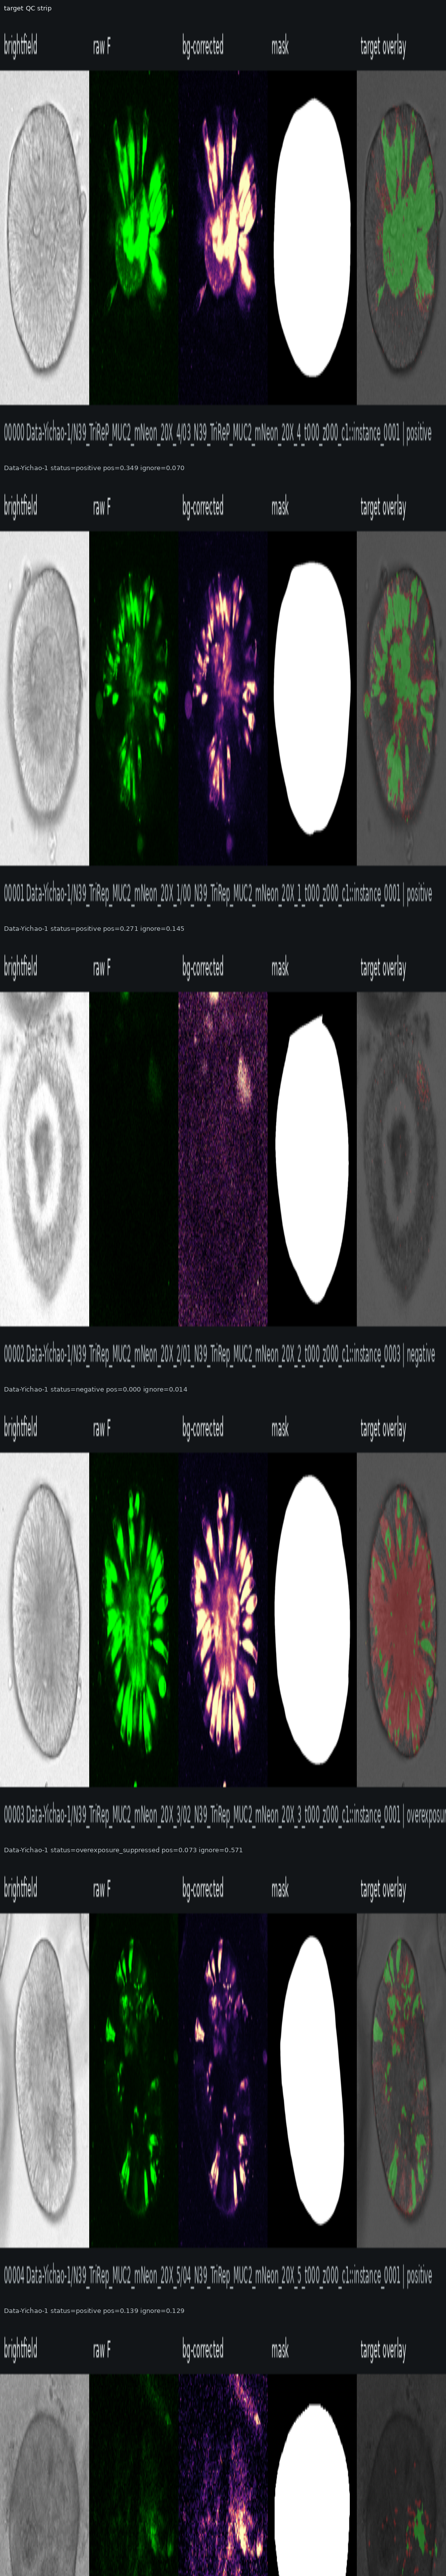
\includegraphics[height=0.82\textheight]{figures/fig2_training_target_qc_gallery.png}
  \caption{Representative excerpt from the training-target quality-control gallery. Columns show the brightfield crop, raw fluorescence, cleaned fluorescence target, and support representation used to define the learning target.}
\end{figure}

\section*{Model and Objective}

The model is a hybrid U-Net style image-to-image network with 256 pixel inputs and one output channel. The input channel count is three: brightfield, organoid mask, and distance map. Training used CUDA with batch size 12, base channels 32, dropout 0.05, learning rate \(1.5\times10^{-4}\), weight decay \(2\times10^{-4}\), and 500 epochs. Each epoch sampled 20,000 training rows with a balanced sampler.

The target is a clipped, normalized, one-channel, noise-suppressed fluorescence signal in \([0,1]\). The loss combines continuous regression with support-aware terms:
\[
\mathcal{L}
= \mathcal{L}_{1,w}
+0.25\,\mathcal{L}_{\mathrm{MSE},w}
+0.5\,\mathcal{L}_{\mathrm{softDice}}
+\mathcal{L}_{\mathrm{focal}}
+0.2\,\mathcal{L}_{\mathrm{total}}
+0.08\,\mathcal{L}_{\mathrm{background}}.
\]
This design avoids forcing the network to learn only a hard binary mask. The continuous target keeps fluorescence intensity information, while soft-Dice and focal support losses prevent sparse positive fluorescent regions from being overwhelmed by background pixels.

\section*{Metrics}

\begin{table}[H]
  \centering
  \caption{Metric interpretation. F1 is the easiest region-detection number; total ratio and log-total correlation explain expression-scale behavior.}
  \resizebox{\textwidth}{!}{\begin{tabular}{@{}lll@{}}
\toprule
Metric & What it measures & Practical interpretation \\
\midrule
F1 best & Best fluorescent-support F1 over thresholds & Main intuitive region-detection accuracy \\
F1 at 0.2 & F1 at the fixed support threshold used in reports & Practical operating-point accuracy \\
Total ratio & Sum of predicted fluorescence divided by true sum & Values near 1 mean calibrated total expression \\
Log-total r & Correlation of log total fluorescence per instance & Whether bright/dim organoids are ranked correctly \\
Pearson & Pixel-level continuous correlation & Fine spatial intensity agreement \\
Positive Pearson & Correlation only inside true positive fluorescence pixels & Quality of intensity prediction inside signal regions \\
\bottomrule
\end{tabular}
}
\end{table}

\section*{Performance}

\begin{table}[H]
  \centering
  \caption{Main validation, internal-test, and external-test performance. The max-projection external row is included as a comparison baseline.}
  \resizebox{\textwidth}{!}{\begin{tabular}{@{}lrrrrrrr@{}}
\toprule
Evaluation set & Rows & Pearson & Pos. Pearson & F1 best & F1 at 0.2 & Total ratio & Log-total r \\
\midrule
Validation, best epoch 210 & 62,814 & 0.449 & 0.230 & 0.477 & 0.447 & 1.016 & 0.587 \\
Validation, epoch 500 & 62,814 & 0.442 & 0.233 & 0.476 & 0.432 & 0.976 & 0.539 \\
Internal test, Data 1--10 & 11,562 & 0.189 & 0.180 & 0.225 & 0.129 & 0.466 & 0.358 \\
External test, Data-Yichao-11 & 7,489 & 0.333 & 0.041 & 0.454 & 0.418 & 1.135 & 0.580 \\
External test, Data-Yichao-11 max projection & 420 & 0.288 & -0.020 & 0.482 & 0.429 & 0.828 & 0.355 \\
\bottomrule
\end{tabular}
}
\end{table}

The best per-z validation checkpoint occurred at epoch 210 with support-best F1 \(=0.477\), fixed-threshold F1 \(=0.447\), and total intensity ratio \(=1.016\). The final epoch retained similar validation performance but was selected for the external last-epoch evaluation in the finished pipeline.

The external Data-Yichao-11 result is the most important deployment-like number. The per-z model reached support-best F1 \(=0.454\), fixed-threshold F1 \(=0.418\), and total intensity ratio \(=1.135\). This means the model roughly finds fluorescent regions and estimates the total fluorescence scale, but it is not yet a pixel-perfect fluorescence reconstruction model.

The internal Data 1--10 test split has lower F1 than the external holdout. This indicates that the split contains harder or distribution-shifted examples. For practical interpretation, the report should not reduce the model to one number; both internal and external behavior should be inspected.

\begin{figure}[H]
  \centering
  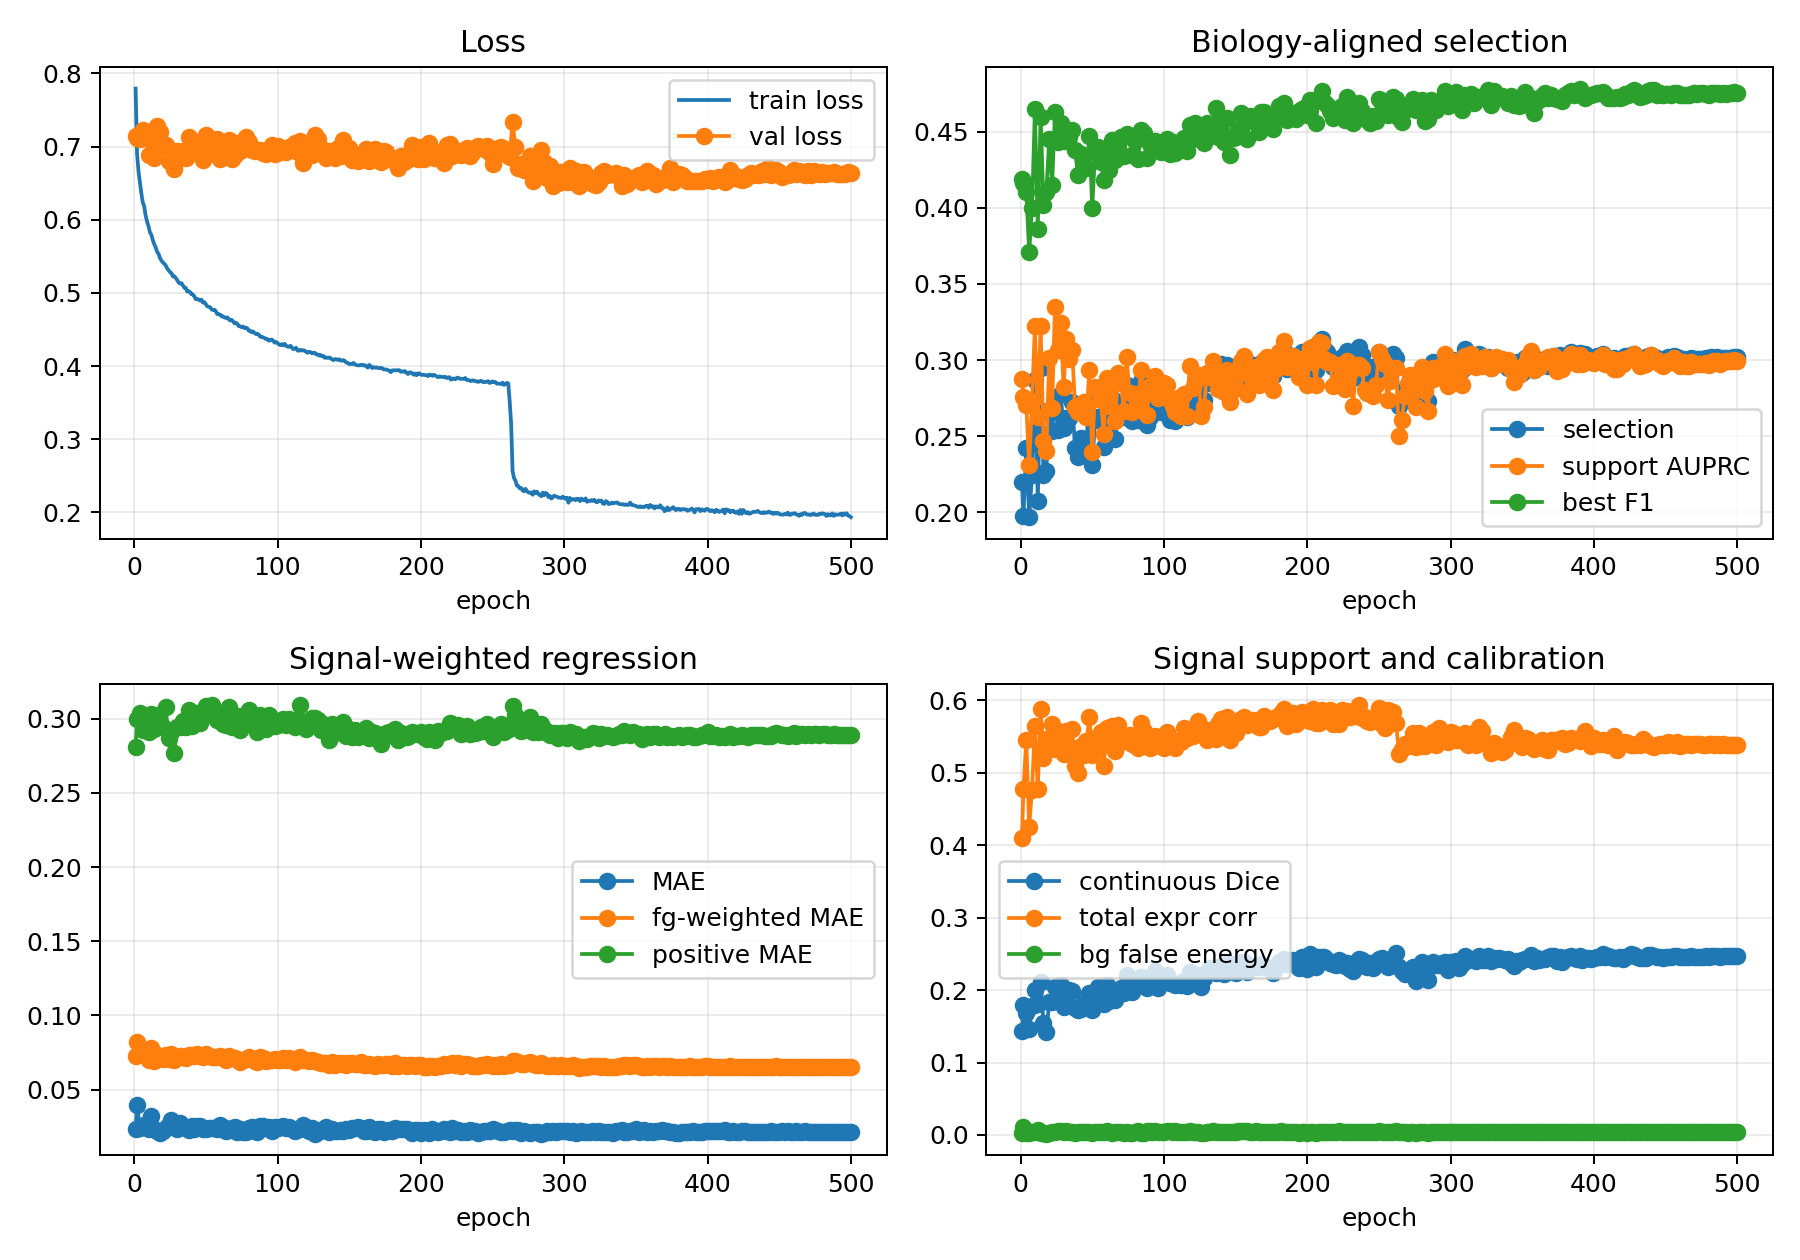
\includegraphics[width=\textwidth]{figures/fig1_per_z_training_metrics.png}
  \caption{Training and validation curves for the completed 500-epoch per-z run.}
\end{figure}

\section*{Prediction Visualizations}

\begin{figure}[H]
  \centering
  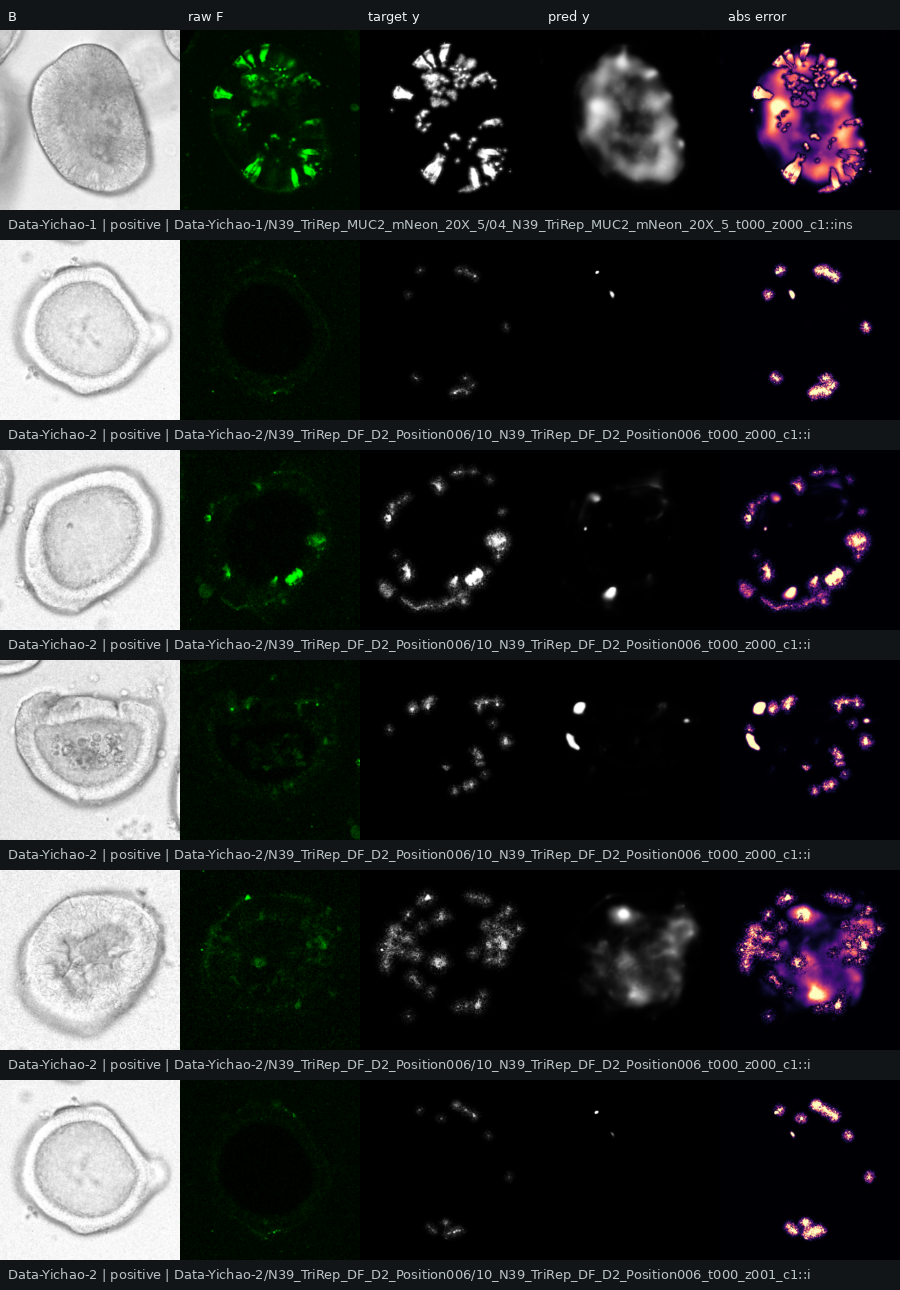
\includegraphics[height=0.82\textheight]{figures/fig3_internal_test_panel.png}
  \caption{Internal test panel from the per-z model. This panel uses held-out Data 1--10 test rows.}
\end{figure}

\begin{figure}[H]
  \centering
  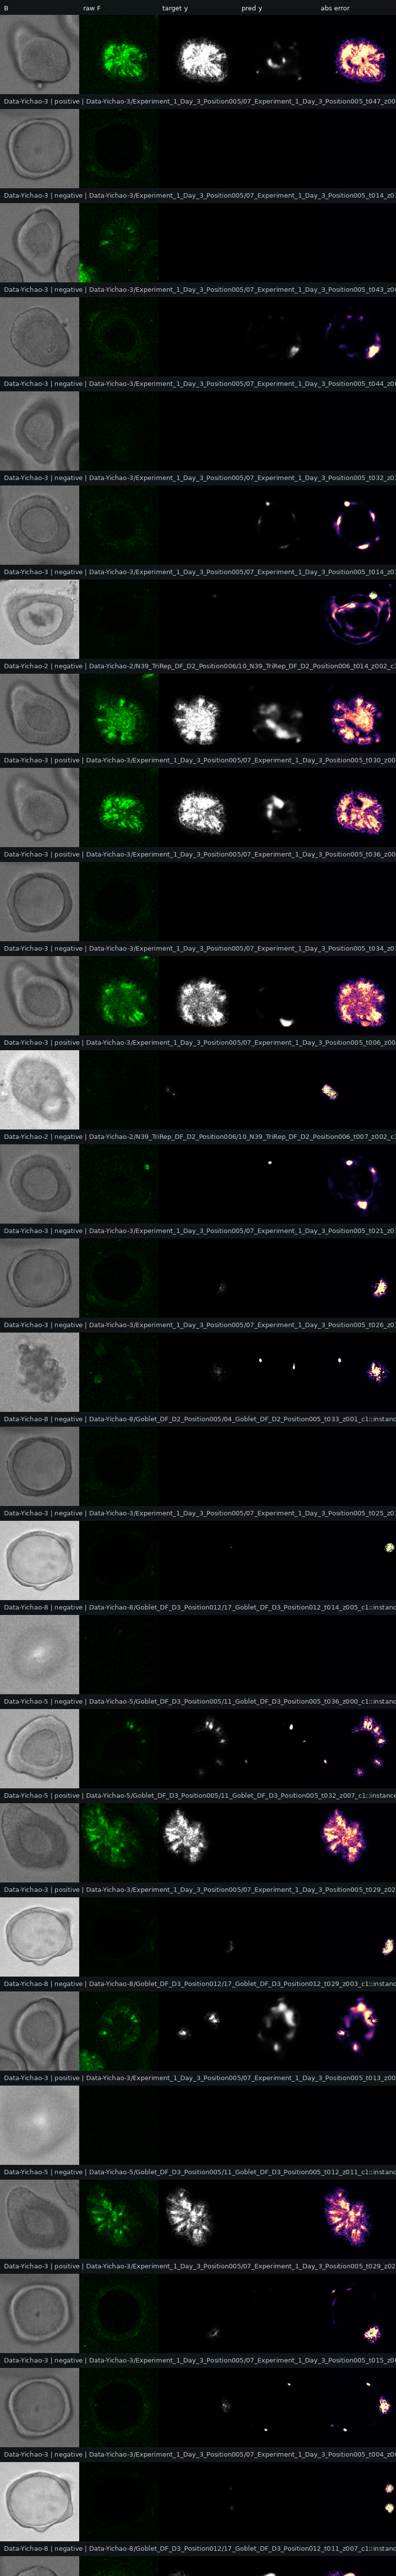
\includegraphics[height=0.82\textheight]{figures/fig4_internal_test_gallery.png}
  \caption{Representative excerpt from the random internal-test gallery. Visual inspection is important because region F1 and pixel correlation capture different failure modes.}
\end{figure}

\begin{figure}[H]
  \centering
  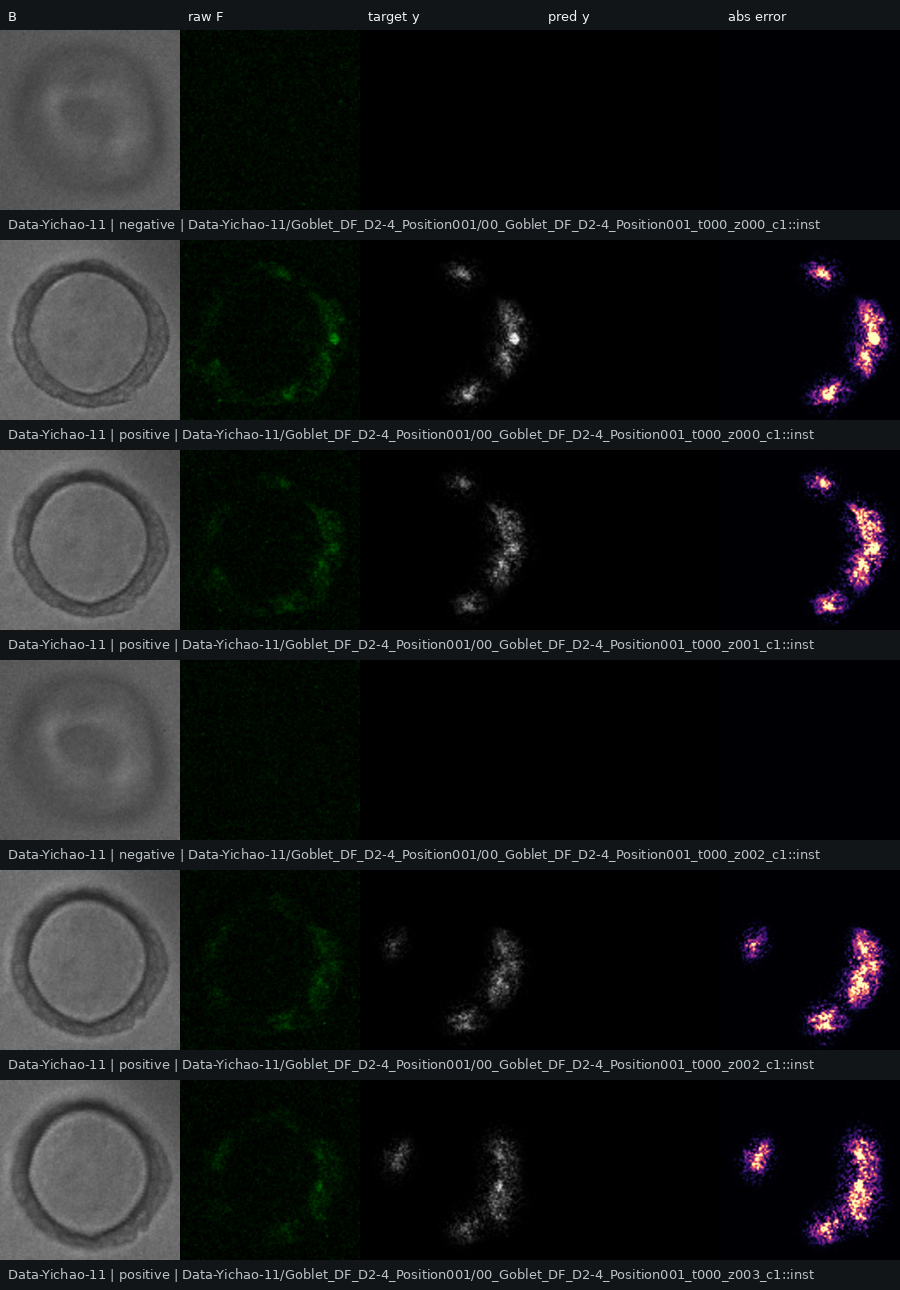
\includegraphics[height=0.82\textheight]{figures/fig5_external_data11_panel.png}
  \caption{External Data-Yichao-11 prediction panel. Data-Yichao-11 was never used during training or validation.}
\end{figure}

\begin{figure}[H]
  \centering
  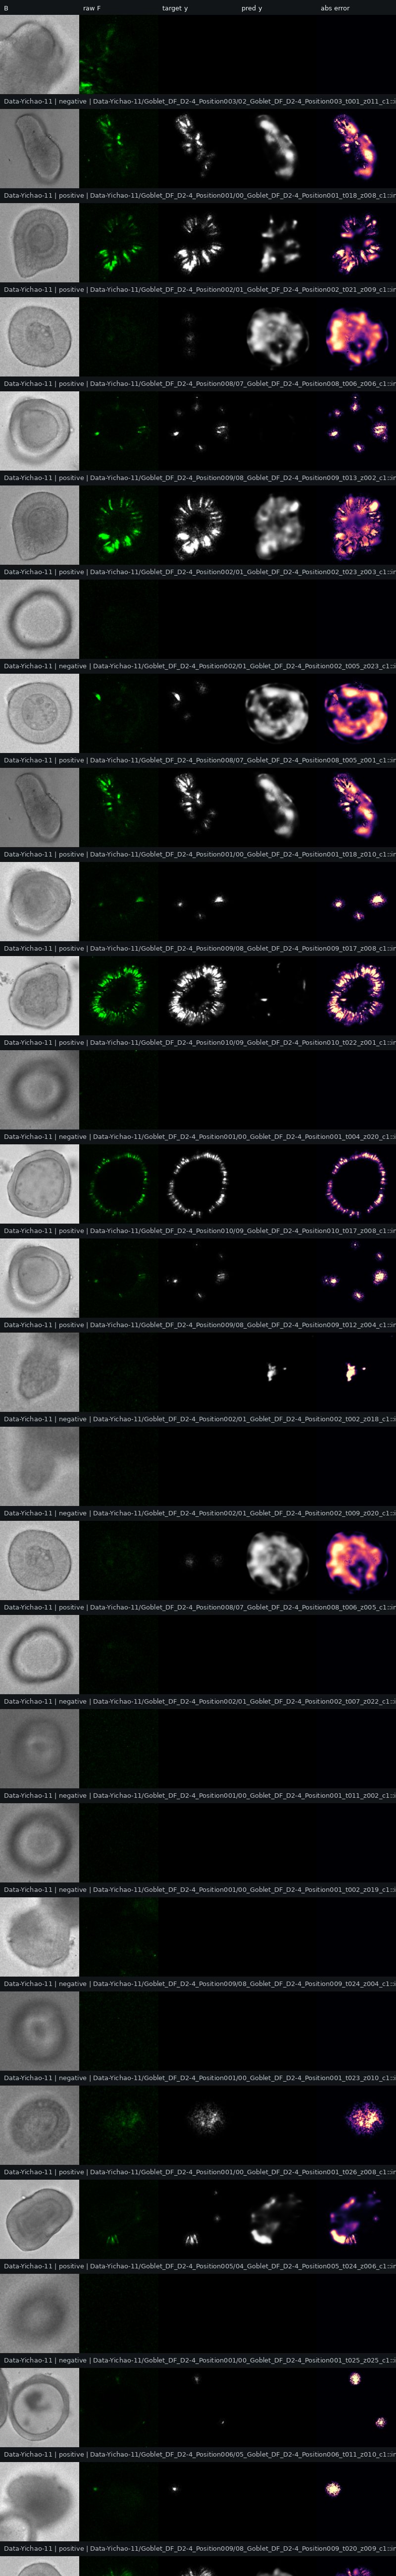
\includegraphics[height=0.82\textheight]{figures/fig6_external_data11_gallery.png}
  \caption{Representative excerpt from the random external Data-Yichao-11 gallery. The model often identifies the correct fluorescent-positive areas at coarse scale, while detailed intensity remains imperfect.}
\end{figure}

\begin{figure}[H]
  \centering
  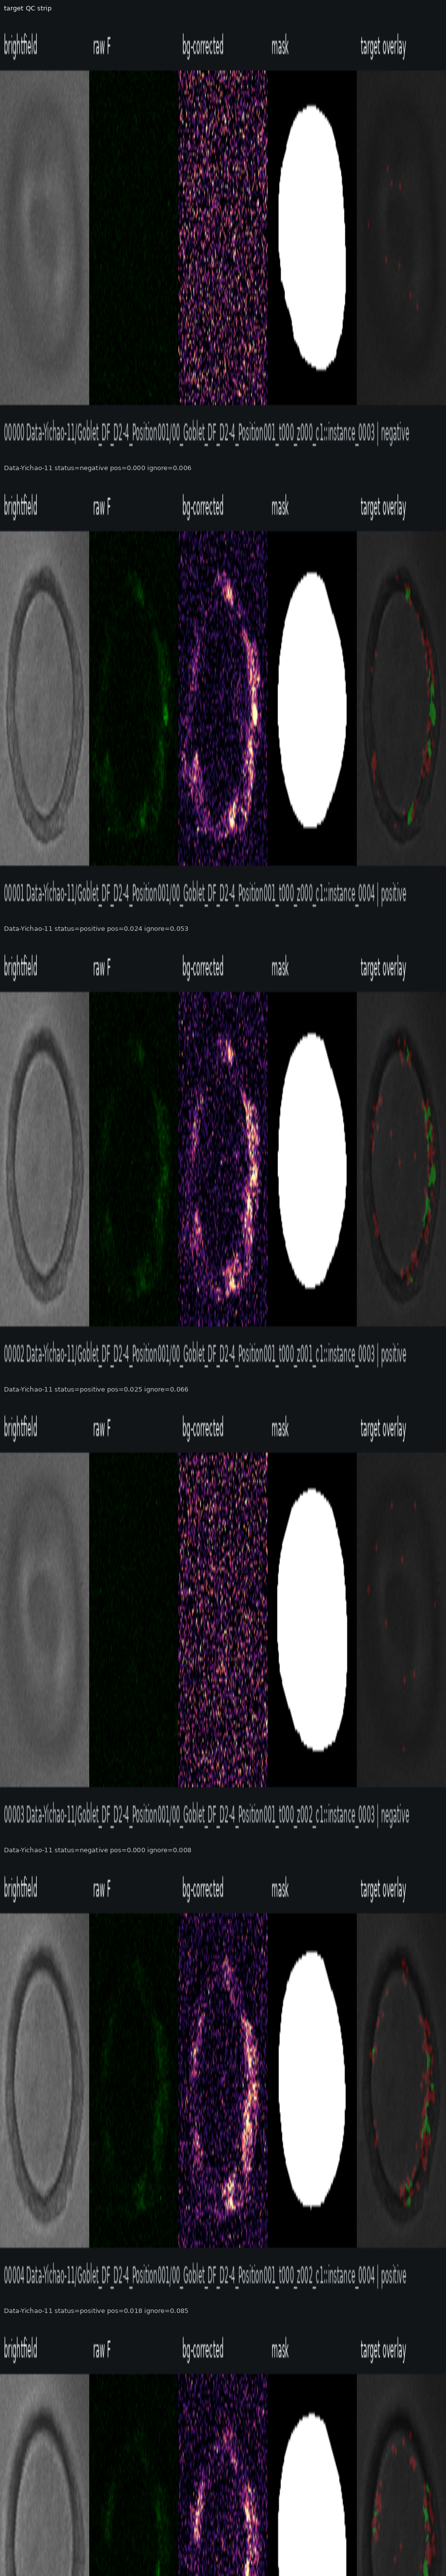
\includegraphics[height=0.82\textheight]{figures/fig7_external_data11_target_qc.png}
  \caption{Representative excerpt from the external Data-Yichao-11 target QC gallery. This shows the fluorescence-derived targets that the model is evaluated against.}
\end{figure}

\section*{Projection Comparison}

The max-projection experiment compresses all z-planes into one projected instance per time/position. It has fewer samples but a cleaner single-image target. On Data-Yichao-11, max projection reached support-best F1 \(=0.482\), slightly higher than the per-z model's \(0.454\). However, its total intensity ratio was \(0.828\), while the per-z model was \(1.135\), and the per-z model had stronger total-intensity log correlation on Data-Yichao-11 (\(0.580\) versus \(0.355\)).

\begin{figure}[H]
  \centering
  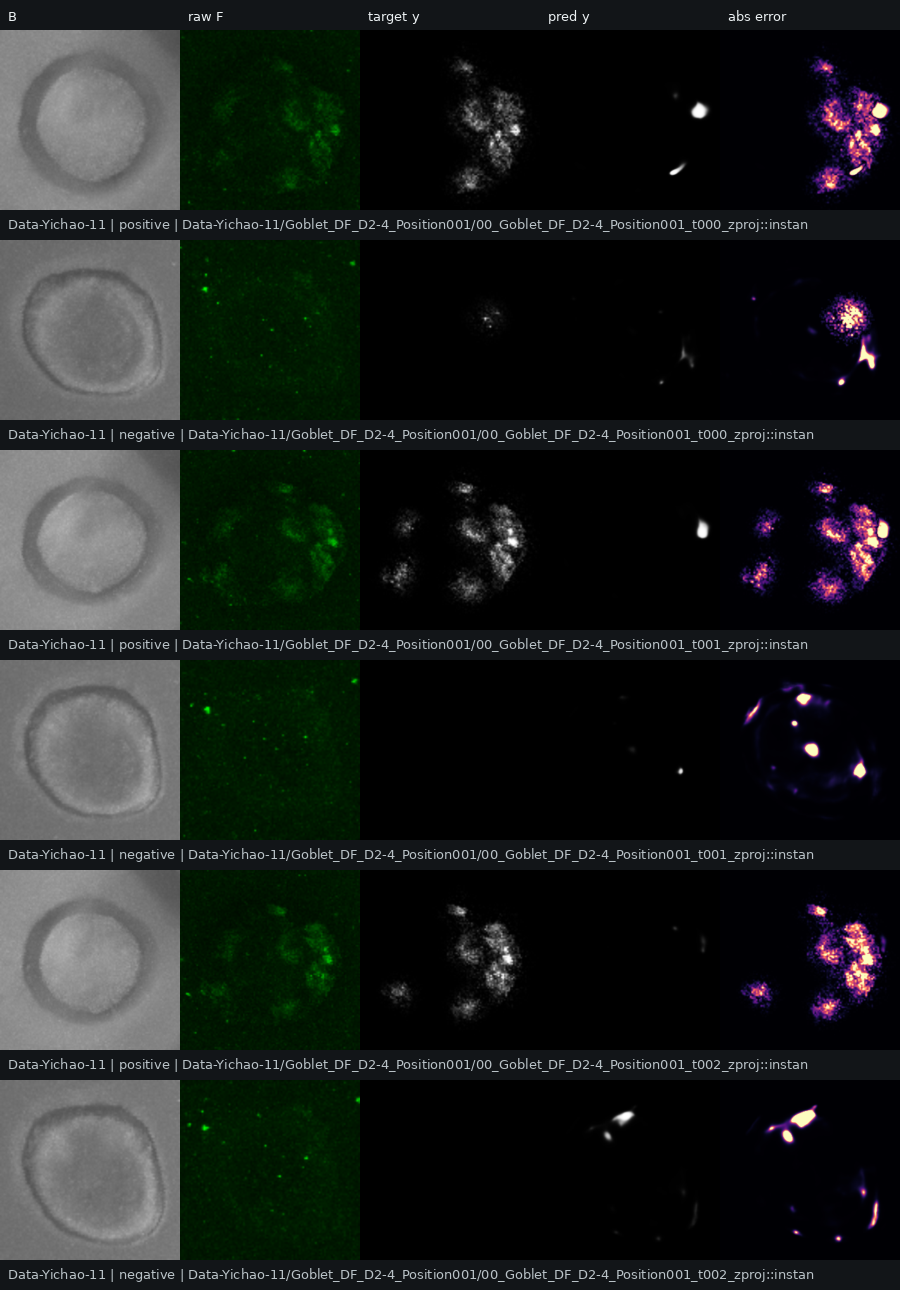
\includegraphics[height=0.82\textheight]{figures/fig8_max_projection_data11_panel.png}
  \caption{External Data-Yichao-11 max-projection comparison panel. Projection can improve region F1 but discards z-level structure.}
\end{figure}

\section*{Interpretation and Next Step}

The current result has value. The external F1 of \(0.454\) is much higher than the \(0.071\) positive support prevalence, and total fluorescence is close to the correct scale. The model is therefore learning a non-random brightfield-to-fluorescence association.

The main weakness is not whether the model learns anything; it does. The weakness is that detailed positive-pixel intensity correlation remains low, especially on external Data-Yichao-11. The next improvement should keep the current continuous-plus-support target design, but improve calibration and temporal consistency. For future-expression prediction, the best route is to use this B2F model as a representation/auxiliary objective and combine it with time-aware organoid trajectories rather than relying on a single same-time pixel prediction alone.

\section*{Artifact Paths}

\begin{itemize}
\item Per-z summary: \path{/home/lachlan/ProjectsLFS/OrganoidAgent/analysis-outputs/yichao_per_z_b2f_pipeline/summary.md}
\item Per-z run root: \path{/home/lachlan/ProjectsLFS/OrganoidAgent/analysis-outputs/yichao_fluorescence_continuous/runs/per_z_1to10_hybrid_unet_v1_500}
\item External Data-Yichao-11 metrics: \path{/home/lachlan/ProjectsLFS/OrganoidAgent/analysis-outputs/yichao_external_tests/Data-Yichao-11_per_z/evaluation/Data-Yichao-11_per_z_last_epoch_external_metrics.json}
\item Markdown reference: \path{/home/lachlan/ProjectsLFS/OrganoidAgent/references/Yichao/per_z_b2f_performance_report.md}
\end{itemize}

\end{document}
